\documentclass[10pt]{beamer}

\usepackage[english]{babel}
\usepackage[utf8]{inputenc}
\usepackage{amssymb}
\usepackage{amsthm}
\usepackage[all]{xy}
\usepackage{graphicx}
\usepackage{tikz}
\usetikzlibrary{trees}

%% Stuff
\renewcommand{\le}{\leqslant}
\renewcommand{\ge}{\geqslant}  % comme François le demande...
\newcommand{\blue}[1]{\textcolor{blue}{#1}}  % colouring
%% Algèbre
\newcommand{\clot}[1]{\bar{#1}}  % clôture algèbrique
\newcommand{\card}[1]{\# #1}  % cardinalité d'un ensemble
\DeclareMathOperator{\car}{char}  % caractéristique d'un corps
\DeclareMathOperator{\Frac}{Frac}  % corps des fractions
\newcommand{\Z}{\mathbb{Z}}  % les entiers
\newcommand{\K}{\mathbb{K}}  % un corps
\newcommand{\LK}{\mathbb{L}}  % encore un corps
\newcommand{\U}{\mathbb{U}}  % encore un corps
\newcommand{\F}{\mathbb{F}}  % un corps fini
\newcommand{\Q}{\mathbb{Q}}  % les rationnels
\newcommand{\R}{\mathbb{R}}  % les réels
\newcommand{\C}{\mathbb{C}}  % les complexes
\newcommand{\isom}{\cong}  % isomorphisme de corps
\newcommand{\frob}{\varphi}  % fröbenius
\DeclareMathOperator{\Gal}{Gal}  % groupe de Galois
\DeclareMathOperator{\Tr}{Tr}  % trace
\DeclareMathOperator{\PTr}{PTr}  % pseudotrace
\DeclareMathOperator{\Norm}{N} % norme
\newcommand{\euler}{\phi}  % indicatrice d'Euler
\DeclareMathOperator{\ord}{ord}  % l'ordre d'un élément
\newcommand{\AS}[1]{\mathcal{#1}}  % la police des polynômes d'AS
\DeclareMathOperator{\rev}{rev}  % le reverse d'un polynôme
%% Courbes
\DeclareMathOperator{\Jac}{Jac}  % la jacobienne
\newcommand{\Proj}{\mathbb{P}}  % espace projectif
\newcommand{\0}{\mathcal{O}}  % point de base d'une courbe
\newcommand{\ecpoint}[3]{[#1:#2:#3]}  % un point d'une courbe
\newcommand{\isog}[1]{\mathcal{#1}}  % la police des isogénies
\newcommand{\I}{\isog{I}}  % une isogénie I
\newcommand{\Hasse}{H}  % l'invariant de Hasse
\newcommand{\divpol}{f}  % polynôme de division
%% Autre
\newcommand{\tildO}{\tilde{O}}  % la notation O~ qui oublie les log
\newcommand{\Mint}{\mathrm{\sf M}_\text{int}}  % fonction de multiplication
\newcommand{\Mpol}[1][]{\mathrm{\sf M}_\text{pol}^{#1}}  % fonction de multiplication
\newcommand{\Mult}[1][]{\mathrm{\sf M}_{#1}}  % fonction de multiplication
\newcommand{\Push}{\mathrm{\sf P}}  % fonction de push-down
\newcommand{\Lift}{\mathrm{\sf L}}  % fonction de lift-up
\newcommand{\Trace}{\mathrm{\sf T}}  % fonction de trace
\newcommand{\Frob}{\mathrm{\sf F}}  % fonction de frobenius itéré
\newcommand{\Ptr}{\mathrm{\sf PT}}  % fonction de pseudo-trace
\newcommand{\ModComp}{\mathrm{\sf C}}  % fonction de composition modulaire
\newcommand{\alg}[1]{\textsf{#1}}  % la police des algorithmes
\newcommand{\wrt}{\dashv}  % appartenance forte, a\wrt A signifie que a est représenté comme un élément de A
\DeclareMathOperator{\op}{op}  % une opération

\newenvironment{algorithm}[3]{\begin{center}\begin{minipage}{0.85\textwidth}
      \sf
      \rule{\textwidth}{0.2pt}\\
      \makebox[\textwidth][c]{\textbf{#1}}\\
      \rule[0.5\baselineskip]{\textwidth}{0.2pt}\\
      \textbf{Input~~} #2\\
      \textbf{Output} #3
      \smallskip
      \begin{enumerate}
}{\end{enumerate}
      \rule{\textwidth}{0.2pt}
\end{minipage}\end{center}}

% beamer-specific
%\setbeamertemplate{theorem begin}{
%  \begin{\inserttheoremblockenv}{
%      Théorème
%      \ifthenelse{\equal{\inserttheoremaddition}{}}
%		 {}
%		 {(\inserttheoremaddition)}    
		 %  \ifx\inserttheoremaddition\@empty\else\ (\inserttheoremaddition)\fi
%    }
%}

\mode<presentation>{%
  \usetheme[]{Madrid}
  \usefonttheme[onlymath]{serif}
  \usecolortheme{crane}
% \usecolortheme{rose}
}


\title[Computing isogenies in small characteristic]{Isogeny computation in small characteristics}
\author[L.~De~Feo]{L.~De~Feo}
\institute[TANC, LIX]{INRIA Projet TANC, LIX École Polytechnique, France}
\date[ECC, Calgary, August 25, 2009]{Elliptic Curve Cryptography\\August 25, 2009\\University of Calgary}


%% \AtBeginSection[]
%% {
%%   \begin{frame}<beamer>
%%     \frametitle{Plan}
%%     \tableofcontents[currentsection]
%%   \end{frame}
%% }


\begin{document}

\begin{frame}
  \titlepage
\end{frame}

%%

\begin{frame}
  \frametitle{Compute isogenies}

  \vspace{-1mm}

  \begin{block}{What?}
    \centering
    (Separable) isogenies: (separable) non-constant regular maps of
    elliptic curves that are group homomorphism
    
    \begin{itemize}
    \item Finite kernel, onto, given by rational fractions.
    \end{itemize}
  \end{block}

  \vspace{-1mm}

  \begin{block}{Why?}
    \begin{columns}[T]
      \begin{column}{0.53\textwidth}
        \begin{itemize}
        \item Point couting.
        \item Prove hardness of discrete logarithm.
        \item Move discrete logarithms to easier curves.
        \end{itemize}
      \end{column}
      \begin{column}{0.46\textwidth}
        \begin{itemize}
        \item Speed up point multiplication.
        \item Hide weak curves behind chains of isogenies.
        \item Define hash functions.
        \end{itemize}
      \end{column}
    \end{columns}
  \end{block}

  \vspace{-1mm}

  \begin{block}{
	\begin{overprint}
	\onslide<1> Multiplication	
	\onslide<2> Frobenius endomorphism
	\onslide<3> Separable isogenies, odd degree (simplified Weierstrass model)
	\onslide<4-5> Normalised (or strict) isogenies
	\end{overprint}
	}
    \begin{overprint}
      \onslide<1>
      \[\begin{aligned}
	{}[m] : E(\clot{\K}) &\rightarrow E(\clot{\K})\\
	                   P &\mapsto [m]P
      \end{aligned}\]
      $\ker\I = E[m]$.

      \onslide<2>
      \[\begin{aligned}
	\frob : E(\clot{\K}) &\rightarrow E(\clot{\K})\\
	               (X,Y) &\mapsto (X^q,Y^q)
      \end{aligned}\]
      $\ker\frob = \{\0\}$.

      \onslide<3-5>
      \[\quad\I(X,Y) = \left(\frac{g(X)}{h^2(X)},
      \only<3-4>{\alert<4>{c}}Y\left(\frac{g(X)}{h^2(X)}\right)'\right)\]
      $\;\ell\;=\;\deg\I\;=\;
      \card{\ker\I} \;=\; 2\deg h + 1\;$ odd.
    \end{overprint}
  \end{block}
\end{frame}

%%

\begin{frame}
  \frametitle{Vélu formula}
  
  \begin{block}{Vélu formula for algebraically closed fields}
    \[E : y^2 = x^3 + ax + b\]
    $H$ a subgroup of $E$, then $E/H$ is an elliptic curve. $\I:E\rightarrow E/H$ given by
    \begin{align*}
      &\I(\0_E) = \I(\0_{E/H})\\
      &\begin{aligned}
        \I(P) = \Biggl( &x(P) + \sum_{Q\in H - \{\0_E\}}x(P+Q) - x(Q) \quad,\\
        &y(P) + \sum_{Q\in H - \{\0_E\}}y(P+Q) - y(Q) \Biggr) \text{.}
      \end{aligned}
    \end{align*}

    $E'=E/H$ is recovered through simple formulae. This is a
    normalised isogeny.
  \end{block}

  \begin{block}{Rational isogenies on non-algebraically closed fields}
    \centering Knowing $\qquad h^2(X) = \prod_{Q\in H-\{\0_E\}}\left(X
    - x(Q)\right)\qquad$ is enough.
  \end{block}
\end{frame}

%%

\begin{frame}
  \frametitle{Computing isogenies: which problem?}

  \begin{block}{Modular polynomial}
    \centering
    $\Phi_\ell(j(E),j(E')) = 0\quad$ iff $\;E\;$ $\ell$-isogenous to $\;E'\;$

    \begin{itemize}
    \item Bivariate symmetric polynomial, degree $\ell$, integer coefficients of
      $\tildO(\ell)$ bits.
    \item Computed in $\tildO(\ell^3)$ bit operations (quasi-optimal).
    \end{itemize}
  \end{block}

  \begin{block}{Which problem?}
    \begin{enumerate}
    \item Given $\;E$, find an $\ell$-isogenous curve and an $\ell$-isogeny.
    \item Given $\;E\;$ and $\;E'$, find an $\ell$-isogeny.
    \end{enumerate}
    \begin{itemize}
    \item Traditional solution to 1: find a curve by factoring
      $\Phi_\ell(X,j(E))$, then solve 2.
    \item In SEA one needs 1, other applications require 2.
    \item We'll focus on 2.
    \end{itemize}
  \end{block}
\end{frame}

%%

\begin{frame}
  \frametitle{Computing isogenies in $\C$}

  \begin{block}{Elliptic functions}
    \vspace{-3mm}
    \begin{gather*}
      \xymatrix{
      E \;\isom\; \C/\left(\omega_1\Z + \omega_2\Z\right) \ar[r]^\I &
      \C/\left(\tfrac{\omega_1}{\ell}\Z + \omega_2\Z\right) \;\isom\; E'
      }\\
      \xymatrix{
        z \ar@{|->}[r] & z
      }
    \end{gather*}
  \end{block}
  
  \begin{block}{Weierstrass functions}
    \vspace{-3mm}
    \begin{gather*}
      \wp_E(z) = z^{-2} + \sum_{k=1}^{\infty}c_kz^{2k} \quad\text{with}\\
      c_1 = -\frac{a}{5}, \qquad c_2 = -\frac{b}{7}, 
      \qquad c_k = \frac{3}{(k-2)(2k+3)}\sum_{j=1}^{k-2}c_jc_{k-1-j}
    \end{gather*}

    \vspace{-3mm}
    \begin{columns}
      \begin{column}{0.4\textwidth}
        \centering
        and they verify
      \end{column}
      \begin{column}{0.6\textwidth}
        \begin{equation*}
          \left\{\begin{aligned}
            \wp_E'^2 &= 4\wp_E^3 + 4a\wp_E + 4b\wp_E \text{,}\\
            \wp_{E'}(z) &=
            \sum_{i=0}^{\ell-1}\wp_E\left(z+i\tfrac{\omega_1}{\ell}\right) -
            \wp_E\left(i\tfrac{\omega_1}{\ell}\right)
            \text{.}
          \end{aligned}\right.
        \end{equation*}
      \end{column}
    \end{columns}
  \end{block}
  
\end{frame}

%%

\begin{frame}
  \frametitle{The large characteristic case}

  \vspace{-1mm}
  
  \begin{block}{Weierstrass functions}
    \vspace{-3mm}
    \begin{gather*}
      \wp_E(z) = z^{-2} + \sum_{k=1}^{\infty}c_kz^{2k} \quad\text{with}\\
      c_1 = -\frac{a}{5}, \qquad c_2 = -\frac{b}{7}, 
      \qquad c_k = \alert<1>{\frac{3}{(k-2)(2k+3)}}\sum_{j=1}^{k-2}c_jc_{k-1-j}
    \end{gather*}
    division by zero when $2k+3 \ge p$.
  \end{block}

  \begin{block}{Large characteristic algorithms \uncover<2>{\alert{*Only work for normalised isogenies}}}
    Work with truncated power series with precision $\ll \frac{p}{2}$.
    \begin{itemize}
    \item['91] Charlap, Coley, Robbins\uncover<2>{\alert{*}} \hfill $O(\ell^2)$
    \item['92] Elkies \hfill $\tildO(\ell^2)$
    \item['92] Atkin \hfill $\tildO(\ell^2)$
    \item['98] Elkies \hfill $\tildO(\ell^2)$
    \item['08] Bostan, Morain, Salvy, Schost\uncover<2>{\alert{*}} \hfill $\tildO(\ell)$
    \end{itemize}
  \end{block}

\end{frame}

%%

\begin{frame}
  \frametitle{Using $p$-adics: Lercier-Sirvent}

  \begin{block}{Weierstrass functions}
    \vspace{-3mm}
    \begin{gather*}
      \wp_E(z) = z^{-2} + \sum_{k=1}^{\infty}c_kz^{2k} \quad\text{with}\\
      c_1 = -\frac{a}{5}, \qquad c_2 = -\frac{b}{7}, 
      \qquad c_k = \alert{\frac{3}{(k-2)(2k+3)}}\sum_{j=1}^{k-2}c_jc_{k-1-j}
    \end{gather*}
  \end{block}

  \begin{block}{Lercier, Sirvent 2009}
    Work in the $p$-adics to avoid divisions by zero.
    \begin{itemize}
    \item Lift $\;E\;$ to $\;\bar{E}\;$ in $\;\Q_q\;$.
    \item Problem: the lift of $\;E'\;$ is not necessarily normalised.
    \item Lift $\;\Phi_\ell$, factor $\;\bar{\Phi}_\ell(X,j(\bar{E}))\;$ to
      obtain a normalised $\;\bar{E}'$,
    \item use BMMS to compute the lifted isogeny, then reduce.
    \end{itemize}
    Works for any $p$, complexity $\tildO(\ell^3)$, but solves problem
    1 directly.
  \end{block}
\end{frame}

%%

\begin{frame}
  \frametitle{Using the $p$-torsion}

  \begin{block}{Other algorithms}
    \begin{itemize}
    \item['94] Couveignes I \hfill $O(\ell^3)$
    \item['96] $p=2$, Lercier \hfill $\Omega(\ell^3)$ ?
    \item['96] Couveignes II (+ D.F.) \hfill $\tildO(\ell^2)$
    \end{itemize}
  \end{block}
  
  \begin{block}{Couveignes I}
    \begin{itemize}
    \item Use formal groups to develop at infinity.
    \end{itemize}
  \end{block}
\end{frame}

%%

\begin{frame}
  \frametitle{Using the $p$-torsion}

  \begin{block}{Other algorithms}
    \begin{itemize}
    \item['94] Couveignes I \hfill $O(\ell^3)$
    \item['96] $p=2$, Lercier \hfill $\Omega(\ell^3)$ ?
    \item['96] Couveignes II (+ D.F., Schost) \hfill $\tildO(\ell^2)$
    \end{itemize}
  \end{block}
  
  \begin{block}{Couveignes II}
    \begin{itemize}
    \item Exploits the cyclic structure of the $p^k$-torsion,
    \item interpolates a polynomial over $E[p^k]$,
    \item reconstructs a rational fraction and tests if it is an isogeny.
    \item Uses fast computer algebra techniques.
    \end{itemize}
  \end{block}
\end{frame}

%%

\begin{frame}
  \frametitle{Structure of the $p^k$-torsion}

  \begin{columns}
    \begin{column}{0.12\textwidth}
      \[\xymatrix{
        \U_k \ar@{-}[d]^p\\
        \U_{k-1} \ar@{--}[d]\\
        \U_{i_0+1} \ar@{-}[d]^p\\
        \U_{i_0} \ar@{--}[d]\\
        \U_1 \ar@{-}[d]^1\\
        \U_0 = \F_q
      }\]
    \end{column}
    \begin{column}{0.86\textwidth}
      \vspace{-2mm}
      \begin{block}{Computing the $p^i$-torsion}
	\begin{itemize}
        \item Iteratively, inverting the map $\;[p]$,
        \item \blue{Voloch Formula:}
          $\;X^p - X = \frac{\sqrt[p]{y_P\beta(x_p)}}{h}$.
        \end{itemize}
      \end{block}

      \vspace{-2mm}
      \begin{definition}[$p^k$-torsion tower]
        $(\F_q = \U_0, \ldots, \U_k)$ is the tower of field extensions of
        minimal degree s.t. for any $i$
        \[E[p^i] \subset E(\U_i)\text{.}\]
      \end{definition}
      
      \vspace{-2mm}
      \begin{theorem}[Structure of $(\U_0, \ldots, \U_k)$]
        There is a $i_0\ge1$ s.t. $\U_{i_0} = \U_1$ and for $i \ge i_0$
        \begin{center}
          $[\U_{i+1}:\U_i] = p$.
        \end{center}
        And $\;[\U_1:\U_0]\;$ divides $\;p-1$.
      \end{theorem}
    \end{column}
  \end{columns}
\end{frame}

%%

\begin{frame}
  \frametitle{Summarizing}

  \vspace{-1mm}

  \begin{block}{Couveignes' algorithm}
    \begin{enumerate}
    \item Compute a $p$-torsion point of $E$,
    \item repeatedly apply Voloch formulae to compute $P$, a $p^k$-torsion
      point of $E$,
    \item do the same to compute $P'$, a $p^k$-torsion point of $E'$,
    \item for $i \in [1,\dots,p^k-1]$, $i$ prime to $p$
      \begin{enumerate}
      \item interpolate the polynomial that sends $P$ over $[i]P'$,
      \item deduce a rational fraction and check if its denominator is
        a square.
      \end{enumerate}
    \end{enumerate}
  \end{block}

  \vspace{-1mm}

  \begin{block}{Informal cost analysis}
    \begin{itemize}
    \item To have enough points \blue{$\;\euler(p^k) > 4\ell$}, then
      $\;[\U_k:\F_q] \sim$ \blue{$p^k \sim \ell$}.
    \item Step 1 is easy, step 2 costs \blue{$O(p^k)$}
      operations in the tower.
    \item Step 3 requires factorisation in $\U_k$. Cost is
      \alt<2>{\alert{$O(p^{3k})$}}{\blue{$O(p^{3k})$}} by linear
      algebra.
    \item Steps 4.1 and 4.2 have to be repeated
      \alt<2>{\alert{$\euler(p^k)$}}{\blue{$\euler(p^k)$}} times.
    \item Step 4.1 interpolates a polynomial of degree
      \blue{$\euler(p^k)$} in a field of degree \blue{$p^{k-1}$}. That
      is \alt<2>{\alert{$O(p^{2k})$}}{\blue{$O(p^{2k})$}} by fast
      techniques.  Step 4.2 is some GCDs in $\F_q$, costs
      \blue{$O(p^k)$}.
    \item<2> Total cost is \blue{$\;O(p^{3k}) = O(\ell^3)$}.
    \end{itemize}
  \end{block}
  
\end{frame}

%%

\begin{frame}
  \frametitle{Improving the isomorphism}

  \vspace{-1mm}

  \begin{block}{Couveignes' algorithm}
    \begin{enumerate}
    \item Compute a $p$-torsion point of $E$,
    \item repeatedly apply Voloch formulae to compute $P$, a $p^k$-torsion
      point of $E$,
    \item \alert<1>{do the same to compute $P'$, a $p^k$-torsion point
      of $E'$,}
    \item for $i \in [1,\dots,p^k-1]$, $i$ prime to $p$
      \begin{enumerate}
      \item interpolate the polynomial that sends $P$ over $[i]P'$,
      \item deduce a rational fraction and check if its denominator is
        a square.
      \end{enumerate}
    \end{enumerate}
  \end{block}

  \vspace{-1mm}

  \begin{block}{Informal cost analysis}
    \begin{itemize}
    \item<0> To have enough points \blue{$\;\euler(p^k) > 4\ell$}, then
      $\;[\U_k:\F_q] \sim$ \blue{$p^k \sim \ell$}.
    \item<0> Step 1 is easy, step 2 costs \blue{$O(p^k)$}
      operations in the tower.
    \item<1> \alert{Step 3 requires factorisation in $\U_k$. Cost is
      \blue{$O(p^{3k})$} by linear algebra.}
    \item<1> \cite{Couveignes00} gives an algorithm with cost
      \blue{$O(p^k)$} operations in the tower.
    \item<0> Step 4.1 interpolates a polynomial of degree
      \blue{$\euler(p^k)$} in a field of degree \blue{$p^{k-1}$}. That
      is \blue{$O(p^{2k})$} by fast techniques.  Step 4.2 is some GCDs
      in $\F_q$, costs \blue{$O(p^k)$}.
    \item<0> Total cost is \blue{$\;O(p^{3k}) = O(\ell^3)$}.
    \end{itemize}
  \end{block}
\end{frame}

%%

\begin{frame}
  \frametitle{Artin-Schreier towers}

  \begin{columns}
    \begin{column}{0.3\textwidth}
      \Large\[\xymatrix{
        *+[r]{\U_k = \frac{\U_{k-1}[X_k]}{P_{k-1}(X_k)}}\ar@{-}[d]^p\\
        *+[r]{\U_{k-1}} \ar@{--}[dd]\\
        \\
        *+[r]{\U_{i_0+1} = \frac{\U_0[X_1]}{P_0(X_1)}} \ar@{-}[d]^p\\
        *+[r]{\U_{i_0} = \F_q = \frac{\F_p[X_0]}{Q(X_0)}}
      }\]
    \end{column}
    \begin{column}{0.65\textwidth}
      \begin{block}{Artin-Schreier Towers over finite fields}
        \smallskip
        \begin{center}
          \Large$P_i = X^p - X - \alpha_i$
        \end{center}

        \begin{center}
          We say that $(\U_0,\ldots,\U_k)$ is defined by
          $(\alpha_0,\ldots,\alpha_{k-1})$ over $\U_{i_0}$.
        \end{center}
        \begin{center}
          \alert{ANY} separable extension of degree $p$ can be
          expressed this way
        \end{center}
      \end{block}

      \begin{block}{Voloch formulae}
        Remark that Voloch formulae give rise to an Artin-Schreier
        tower:
        \[X^p - X = \frac{\sqrt[p]{y_P\beta(x_p)}}{h}\]
      \end{block}
    \end{column}
  \end{columns}
\end{frame}

%%

\begin{frame}
  \frametitle{Solving Artin-Schreier equations in Artin-Schreier towers}

  \begin{columns}
    \begin{column}{0.1\textwidth}
      \Large\[\xymatrix{
        \U_k\ar@{-}[d]\\
        \U_{k-1} \ar@{--}[dd]\\
        \\
        \U_1 \ar@{-}[d]\\
        \U_0
      }\]
    \end{column}
    \begin{column}{0.75\textwidth}
      \begin{block}{\cite{Couveignes00}}
        \begin{itemize}
        \item Given $\;\alpha_i\in\U_i\;$ solves
          \[X^p-X=\alpha_i\in\U_i\text{.}\]
        \item By a change of variables, this is equivalent to solve
          \[X^p-X=\beta_i\in\U_{i-1}\text{.}\]
        \item Applies the formula recursively. Complexity is
          \blue{$O(p^i)$}.
        \end{itemize}
      \end{block}

      \begin{block}{Isomorphisms of Artin-Schreier towers}
        \begin{itemize}
        \item Equivalently, the algorithm finds an isomorphisms
          between $(\U_0,\ldots,\U_k)$ and the tower defined by
          $(\alpha_0,\ldots,\alpha_{k-1})$.
        \item If there were a third tower $(\LK_0,\ldots,\LK_k)$ with
          fast arithmetics\dots
        \end{itemize}
      \end{block}
    \end{column}
    \begin{column}{0.1\textwidth}
      \Large\[\xymatrix{
        \U_k'\ar@{-}[d]\\
        \U_{k-1}' \ar@{--}[dd]\\
        \\
        \U_1' \ar@{-}[d]\\
        \U_0'
      }\]
    \end{column}
  \end{columns}
\end{frame}

%%

\begin{frame}
  \frametitle{Solving Artin-Schreier equations in Artin-Schreier towers}

  \Large\[\xymatrix{
    \U_k \ar@{-}[d]\ar[r]      & \LK_k \ar@{-}[d]      & \U_k' \ar@{-}[d]\ar[l]\\
    \U_{k-1} \ar@{--}[dd]\ar[r] & \LK_{k-1} \ar@{--}[dd] & \U_{k-1}' \ar@{--}[dd]\ar[l]\\
    \\
    \U_1 \ar@{-}[dr]\ar[r]     & \LK_1 \ar@{-}[d]      & \U_1' \ar@{-}[dl]\ar[l]\\
                         &\U_0=\LK_0=\U_0'
  }\]
\end{frame}

%%

\begin{frame}
  \frametitle{Improving the arithmetics}

  \vspace{-1mm}

  \begin{block}{Couveignes' algorithm}
    \begin{enumerate}
    \item Compute a $p$-torsion point of $E$,
    \item repeatedly apply Voloch formulae to compute $P$, a $p^k$-torsion
      point of $E$,
    \item do the same to compute $P'$, a $p^k$-torsion point
      of $E'$,
    \item for $i \in [1,\dots,p^k-1]$, $i$ prime to $p$
      \begin{enumerate}
      \item interpolate the polynomial that sends $P$ over $[i]P'$,
      \item deduce a rational fraction and check if its denominator is
        a square.
      \end{enumerate}
    \end{enumerate}
  \end{block}

  \vspace{-1mm}

  \begin{block}{\alert<2>{Informal} cost analysis}
    \begin{itemize}
    \item To have enough points \blue{$\;\euler(p^k) > 4\ell$}, then
      $\;[\U_k:\F_q] \sim$ \blue{$p^k \sim \ell$}.
    \item Step 1 is easy, step 2 costs \blue{$O(p^k)$}
      \alert<2>{operations in the tower}.
    \item \alert<1>{Step 3 requires factorisation in $\U_k$. Cost is
      \blue{$O(p^{k})$} \alert<2>{ops} by \cite{Couveignes00}.}
    \item Steps 4.1 and 4.2 have to be repeated
      \blue{$\euler(p^k)$} times.
    \item Step 4.1 interpolates a polynomial of degree
      \blue{$\euler(p^k)$} in a field of degree \blue{$p^{k-1}$}. That
      is \blue{$O(p^{2k})$} \alert<2>{operations}. Step 4.2 is some GCDs
      in $\F_q$, costs \blue{$O(p^k)$} \alert<2>{ops}.
    \item \uncover<2>{\alert{But how much does it cost \emph{one operation}?}}
    \end{itemize}
  \end{block}
\end{frame}

%%

\begin{frame}
  \frametitle{Fast arithmetics in Artin-Schreier towers}

  \begin{columns}
    \begin{column}{0.1\textwidth}
      \Large\[\xymatrix{
        \U_k\ar@{-}[d]\\
        \U_{k-1} \ar@{--}[dd]\\
        \\
        \U_1 \ar@{-}[d]\\
        \U_0
      }\]
    \end{column}
    \begin{column}{0.85\textwidth}
      \vspace{-3mm}
      \begin{block}{Primitive towers (\cite{DFS09})}
        \begin{itemize}
        \item Find special $(\gamma_0,\ldots,\gamma_{k-1})$ that
          define a tower s.t. $\LK_i = \F_p[x_i]$, where
          $\;x_i^p-x_i-\gamma_{i-1}=0$.
        \item Use univariate representation over $\F_p$ to perform
          fast arithmetics (FFT multiplication, Newton inversion,
          etc.).
        \item Use \cite{Couveignes00} algorithm to move to
          $(\U_0,\ldots,\U_k)$.
        \end{itemize}
      \end{block}
      
      \vspace{-3mm}
      \begin{block}{Level embedding (\cite{DFS09})}
        \begin{itemize}
        \item Express the morphisms between the levels to switch back
          to the multivariate representation.
        \item Going down is easy: bivariate reduction modulo
          $X_i^p-X_i-\gamma_{i-1}$.
        \item Going up much harder: trace formulae, truncated power
          series arithmetics, transposition principle.
        \end{itemize}
      \end{block}

      \vspace{-3mm}
      \begin{block}{Advertisement: \texttt{FAAST}}
        Download this \texttt{C++} library at:
        \blue{\url{http://www.lix.polytechnique.fr/Labo/Luca.De-Feo/FAAST}}
      \end{block}
    \end{column}
  \end{columns}
\end{frame}

%%

\begin{frame}
  \frametitle{Improving the interpolation}

  \vspace{-2mm}

  \begin{block}{Couveignes' algorithm}
    \begin{enumerate}
    \item Compute a $p$-torsion point of $E$,
    \item repeatedly apply Voloch formulae to compute $P$, a $p^k$-torsion
      point of $E$,
    \item do the same to compute $P'$, a $p^k$-torsion point
      of $E'$,
    \item for $i \in [1,\dots,p^k-1]$, $i$ prime to $p$
      \begin{enumerate}
      \item interpolate the polynomial that sends $P$ over $[i]P'$,
      \item deduce a rational fraction and check if its denominator is
        a square.
      \end{enumerate}
    \end{enumerate}
  \end{block}

  \vspace{-2mm}

  \begin{block}{Formal cost analysis}
    \begin{itemize}
    \item To have enough points \blue{$\;\euler(p^k) > 4\ell$}, then
      $\;[\U_k:\F_q] \sim$ \blue{$p^k \sim \ell$}.
    \item Step 1 is easy, step 2 costs \blue{$O(p^k\log_pq)$}
      operations .
    \item Step 3 requires factorisation in $\U_k$. Cost is
      \blue{$O(p^{k}\log_p^2q + \log_p^3q)$}.
    \item Steps 4.1 and 4.2 have to be repeated
      \blue{$\euler(p^k)$} times.
    \item Step 4.1 interpolates a polynomial of degree
      \blue{$\euler(p^k)$} in a field of degree \blue{$p^{k-1}$}. That
      is
      \alt<2>{\alert{$O(p^{2k}\log_pq)$}}{\blue{$O(p^{2k}\log_pq)$}}. Step
      4.2 is some GCDs in $\F_q$, costs \blue{$O(p^k\log_pq)$}.
    \item \alert<1>{All costs in $\F_p$-operations.}
    \end{itemize}
  \end{block}
\end{frame}

%%

\begin{frame}
  \frametitle{Faster interpolation using effective Galois groups}

  \begin{center}
    Interpolation of $\;v_i\mapsto s_i\;$ is defined modulo $T$, where
    \[T(X) = \prod_i (X - v_i)\]
  \end{center}
  
  \vspace{-3mm}
  
  \begin{block}{Lagrange formula}
      \centering
      \begin{onlyenv}<1-5>
      \begin{equation*}
        \only<1>{A(X) = \sum_{i=1}^nv_i\frac{T(X)}{X-v_i}\prod_{j\ne
            i}\frac{1}{v_i-v_j}} \only<2>{A(X) =
          \sum_{i=1}^n\frac{s_i}{T'(v_i)}\cdot\frac{T(X)}{X-v_i}}
        \only<3>{A_1(X) = \frac{s_1}{T'(v_1)(X-v_2)}+\frac{s_2}{T'(v_2)(X-v_1)}}
        \only<4>{A_2(X) = \frac{s_3}{T'(v_3)(X-v_4)}+\frac{s_4}{T'(v_4)(X-v_3)}}
        \only<5>{A(X) = T_2(X)A_1(X) + T_1(X)A_2(X)}
      \end{equation*}
      \end{onlyenv}
      \only<6>{Complexity $\tildO(n)$ operations in the coefficient
        ring.}  \only<7>{Let now $v\in\U_2$,
        $\sigma\in\Gal(\U_2/\U_0)$ and
        $v_i=\sigma^{i-1}(v)$. Rearrange the tree, then
        $T_1',T_2'\in\U_1[X]$ and $T\in\U_0[X]$.}  \only<8-9>{For a
        polynomial $P$ note $P^\sigma$ the action on the coefficients
        of $P$, then} \only<10>{Complexity $\tildO(n)$ operations in $\U_0$.}
  \end{block}

  \begin{block}<2->{Interpolation by chinese remindering}
    \centering
    \begin{tikzpicture}
      \begin{scope}
        [level distance=1cm,
          level 1/.style={sibling distance=4cm},
          level 2/.style={sibling distance=2cm},
          every node/.style={rounded corners,thick,draw=black}]
        \node{\alert<5>{$T(X)$}}
        child { node {\alert<3>{$T_1\only<7->{'}(X)$}}
          child {node {\alert<3>{$X-\alt<7->{v}{v_1}$}}}
          child {node {\alert<3>{$X-\alt<7->{\sigma^2(v)}{v_2}$}}}
        }
        child {node {\alert<4>{\alt<9->{$T_1'(X)^\sigma$}{$T_2\only<7->{'}(X)$}}}
          child {node {\only<-9>{\alert<4>{\alt<8->{$(X-v)^\sigma$}{$X-\alt<7->{\sigma(v)}{v_3}$}}}}}
          child {node {\only<-9>{\alert<4>{\alt<8->{$(X-\sigma^2(v))^\sigma$}{$X-\alt<7->{\sigma^3(v)}{v_4}$}}}}}
        };
      \end{scope}
    \end{tikzpicture}
  \end{block}
\end{frame}

%%

\begin{frame}
  \frametitle{Summarizing}

  \vspace{-2mm}

  \begin{block}{Couveignes' algorithm}
    \begin{enumerate}
    \item Compute a $p$-torsion point of $E$,
    \item repeatedly apply Voloch formulae to compute $P$, a $p^k$-torsion
      point of $E$,
    \item do the same to compute $P'$, a $p^k$-torsion point
      of $E'$,
    \item for $i \in [1,\dots,p^k-1]$, $i$ prime to $p$
      \begin{enumerate}
      \item interpolate the polynomial that sends $P$ over $[i]P'$,
      \item deduce a rational fraction and check if its denominator is
        a square.
      \end{enumerate}
    \end{enumerate}
  \end{block}

  \vspace{-2mm}

  \begin{block}{Formal cost analysis}
    \begin{itemize}
    \item To have enough points \blue{$\;\euler(p^k) > 4\ell$}, then
      $\;[\U_k:\F_q] \sim$ \blue{$p^k \sim \ell$}.
    \item Step 1 is easy, step 2 costs \blue{$O(p^k\log_pq)$}
      operations .
    \item Step 3 requires factorisation in $\U_k$. Cost is
      \blue{$O(p^{k}\log_p^2q + \log_p^3q)$}.
    \item Steps 4.1 and 4.2 have to be repeated
      \blue{$\euler(p^k)$} times.
    \item Step 4.1 costs \alert{$O(p^k\log_pq)$} using the latter
      algorithm. Step 4.2 is some GCDs in $\F_q$, costs
      \blue{$O(p^k\log_pq)$}.
    \item Total cost is \blue{$\;O(\ell^2\log_pq + \ell\log_p^2q + \log_p^3q)$}.
    \end{itemize}
  \end{block}
\end{frame}

%%

\begin{frame}
  \frametitle{Reducing the number of interpolations}

  \begin{block}{Couveignes' algorithm}
    \begin{itemize}
    \item We need $O(p^k)$ interpolations, each sending $P\in E[p^k]$
      over $Q\in E'[p^k]$,
    \item $Q,R\in E'[p^k]$ are conjugates tied by the relation
      $Q=\frob_q^i(P)$ for some $i$.
    \end{itemize}
  \end{block}

  \begin{block}{Using modular composition}
    Let $A_Q$ be the polynomial with coefficients in $\F_q$ sending
    $P$ over $Q$, then
    \[A_Q([j]P) = [j]Q \text{ for every $j$.}\]
    Now let $\;\frob_q(Q) = [\lambda]Q\;$, then $\;A_Q(\frob_q([j]P)) =
    [j][\lambda]Q$.

    So \alert{$\;A_Q\circ\frob_q = A_{[\lambda]Q} \bmod T$}. Solving this
    is \emph{modular composition}.
  \end{block}

  \begin{block}{Modular composition}
    \begin{itemize}
    \item Theoretical complexity \blue{$O(\ell\log_pq)$}, practical
      complexity \blue{$O(\ell^2\log_p^2q)$}\dots
    \item \dots but still much faster than a single interpolation.
    \end{itemize}
  \end{block}
\end{frame}

%%

\section{Benchmarks}

\begin{frame}
  \frametitle{(Old) Timings}

  \begin{columns}
    \begin{column}{0.4\textwidth}
      \begin{itemize}
      \item \texttt{Magma} implementation,
      \item \cite{Cou96} vs. \cite{DF07},
      \item $\F_q = \F_{5^3}$.
      \end{itemize}
    \end{column}
    \begin{column}{0.6\textwidth}
      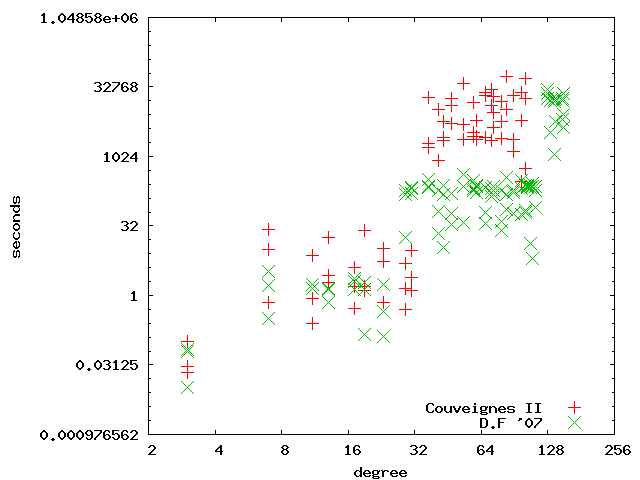
\includegraphics[width=\textwidth]{5}

      \smallskip
      \footnotesize
      \centering
      \begin{tabular}{|l|r|r|}
        \hline
        & [Cou'96] & \cite{DF07}\\
        \hline
        
        Total time           &  $65951$ & $19864$\\
        Compute $E[p^k]$    &           $0,06$\% & $0,5$\%\\
        Compute $E'[p^k]$   &             $28$\% & $89,5$\%\\
        Interpolation &             $71$\% & $9,5$\%\\
        \hline
      \end{tabular}
    \end{column}
  \end{columns}
\end{frame}

%%

\begin{frame}
  \frametitle{Timings}

  
  \begin{columns}
    \begin{column}{0.4\textwidth}
      \begin{itemize}
      \item \texttt{NTL} implemantation of \cite{DFS09} vs.  \texttt{Magma}
        implementation, of \cite{Couveignes00}
      \item $\F_q = \F_{2^{101}}$.
      \end{itemize}
    \end{column}
    \begin{column}{0.6\textwidth}
      \alt<2>{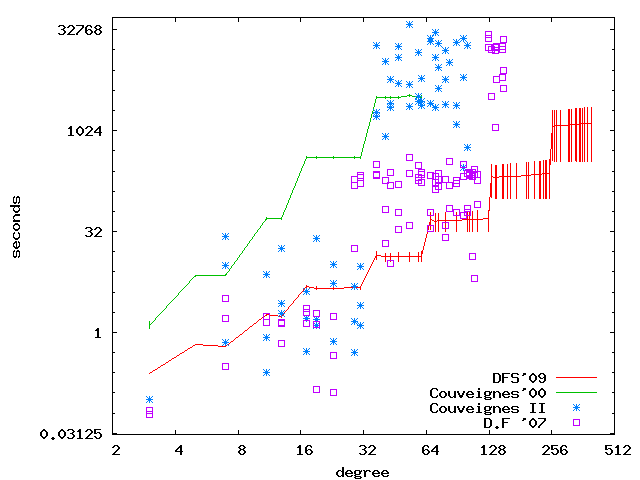
\includegraphics[width=\textwidth]{5+2-101}}
             {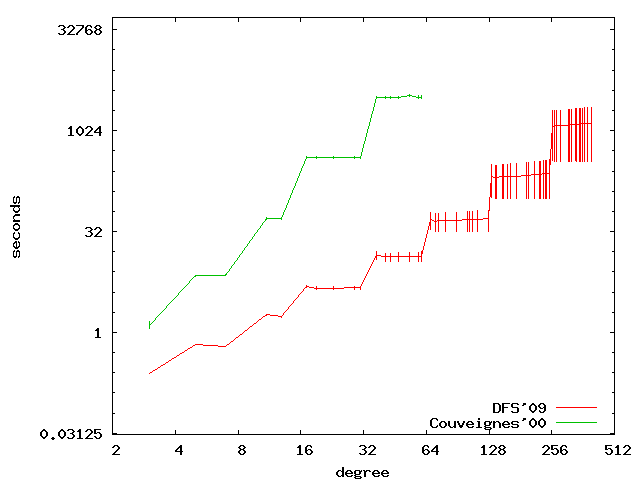
\includegraphics[width=\textwidth]{2-101}}

    \end{column}
  \end{columns}
  
  \smallskip
  \footnotesize
  \centering
  \begin{tabular}{r r r r r r r r}
    \hline
    $\ell$ & $E[p^k]$ & $E'[p^k]$ & Interp & Step 6 & ModComp & Avg tries & Avg loop time\\
    \hline
    31 & 1.3128 & 1.3128 & 1.1058 & 0.00218 & 0.00218 & 64 & 0.279\\
    61 & 3.5454 & 3.5464 & 2.5236 & 0.00783 & 0.00900 & 128 & 2.154 \\
    127 & 9.2975 & 9.3026 & 5.6881 & 0.03147 & 0.03634 & 256 & 17.359 \\
    251	& 23.7984 & 23.7984 & 12.7251 & 0.12415 & 0.14519 & 512 & 137.902 \\
    397 & 59.7439 & 59.7579 & 28.3387 & 0.36822 & 0.58027 & 1024 & 971.254 \\
    \hline
  \end{tabular}
\end{frame}

%%

\begin{frame}
  \frametitle{Timings}

  
  \begin{columns}
    \begin{column}{0.4\textwidth}
      \begin{itemize}
      \item \texttt{NTL} implemantation of \cite{DFS09}
      \item $\F_q = \F_{3^{64}}$.
      \end{itemize}
    \end{column}
    \begin{column}{0.6\textwidth}
      \alt<2>{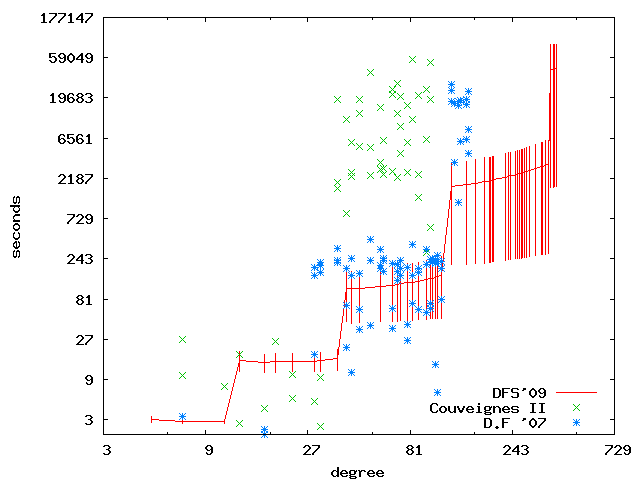
\includegraphics[width=\textwidth]{5+3-64}}
             {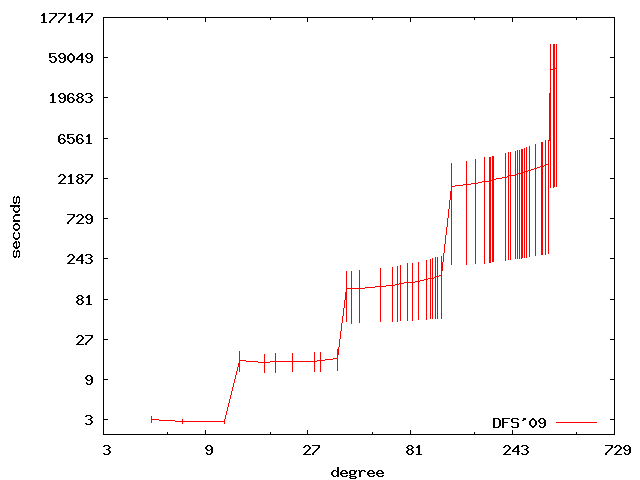
\includegraphics[width=\textwidth]{3-64}}

    \end{column}
  \end{columns}
  
  \smallskip
  \footnotesize
  \centering
  \begin{tabular}{r r r r r r r r}
    \hline
    $\ell$ & $E[p^k]$ & $E'[p^k]$ & Interp & Step 6 & ModComp & Avg tries & Avg loop time\\
    \hline
    11 & 0.6109 & 0.6109 & 0.4669 & 0.0194 & 0.0249 & 13 & 0.58 \\
    37 & 2.3946 & 2.3916 & 2.1066 & 0.1988 & 0.1381 & 40 & 13.48 \\
    113 & 9.8045 & 9.8055 & 8.5377 & 1.7712 & 0.8690 & 121 & 319.47 \\
    359 & 38.3292 & 38.3972 & 34.7147 & 17.5004 & 7.0088 & 364 & 8921.35 \\ 
    389 & 159.8280 & 159.5690 & 147.741 & 45.1558 & 69.9133 & 1093 & 125770.52  \\   
    \hline
  \end{tabular}
\end{frame}

%%

\begin{frame}
  \frametitle{Record Timings!}

  
  \begin{columns}
    \begin{column}{0.4\textwidth}
      \begin{itemize}
      \item \texttt{NTL} implemantation of \cite{DFS09}
      \item $\F_q = \F_{2^{1023}}$.
      \end{itemize}
    \end{column}
    \begin{column}{0.6\textwidth}
      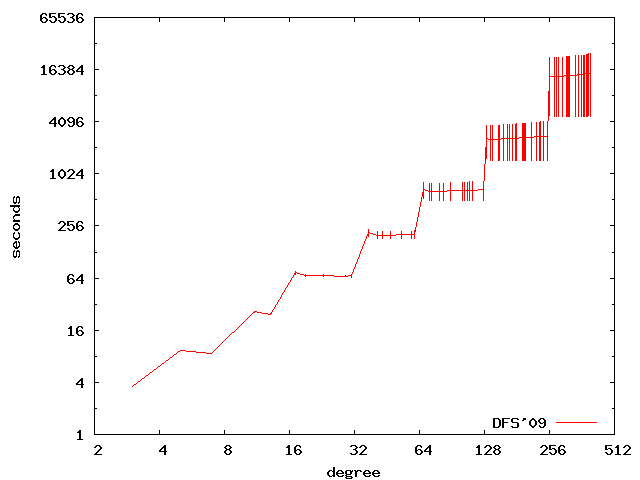
\includegraphics[width=\textwidth]{2-1023}

    \end{column}
  \end{columns}
  
  \smallskip
  \footnotesize
  \centering
  \begin{tabular}{r r r r r r r r}
    \hline
    $\ell$ & $E[p^k]$ & $E'[p^k]$ & Interp & Step 6 & ModComp & Avg tries & Avg loop time\\
    \hline
    31 & 21.182 & 21.174 & 11.597 & 0.0178 & 0.02541 & 64 & 2.768 \\
    61 & 58.656 & 58.665 & 26.826 & 0.0645 & 0.10398 & 128 & 21.576 \\
    127 & 154.357 & 154.296 & 61.202 & 0.2580 & 0.41578 & 256 & 172.503 \\
    251 & 383.773 & 383.861 & 138.428 & 0.9950 & 1.66120 & 512 & 1360.000 \\
    397 & 931.022 & 931.610 & 313.609 & 3.1819 & 6.73608 & 1024 & 10156.011 \\
    \hline
  \end{tabular}
\end{frame}

%%

\begin{frame}
  \frametitle{Ongoing work}

  \begin{block}{Implementation (with F. Morain and E. Schost)}
    \begin{itemize}
    \item \texttt{SAGE} porting of \texttt{FAAST},
    \item \texttt{SAGE} porting of SEA + Lercier + Couveignes II,
    \item comparison with Lercier,
    \item comparison with Lercier-Sirvent.
    \end{itemize}
  \end{block}

  \begin{block}{Theory}
    \begin{itemize}
    \item Try a $p$-adic version of Couveignes II + BMSS08 to reduce
      the number of tries in the final loop,
    \item Improve Lercier-Sirvent and make it the best algorithm for
      this problem.
    \end{itemize}
  \end{block}
\end{frame}

%%

\begin{frame}
  \begin{center}
    \Large
    \textbf{Thanks}
  \end{center}
\end{frame}

%%
%%

\begin{frame}
  \frametitle{Bibliography}

  \begin{thebibliography}{1}
    \beamertemplatebookbibitems
    
  \bibitem[BSS1]{BSS1} I.~Blake, G.~Seroussi \& N.~Smart
    \newblock \emph{Elliptic Curves in Cryptography}
    \newblock LMS 265, Cambridge University Press, 1999
    
  \bibitem[BSS2]{BSS2} (edited by) I.~Blake, G.~Seroussi \& N.~Smart
    \newblock \emph{Advances in Elliptic Curve Cryptography}
    \newblock LMS 317, Cambridge University Press, 2005
        
  \bibitem[Mil]{MIL} J.S.~Milne.
    \newblock \emph{Elliptic curves}.
    \newblock BookSurge Publishers, ISBN 1-4196-5257-5, 2006.

  \bibitem[Sil]{SIL1} J.H.~Silverman
    \newblock \emph{The Arithmetic of Elliptic Curves}
    \newblock GTM 106, Springer-Verlag, 1986
        
  \end{thebibliography}
\end{frame}

\begin{frame}
  \frametitle{Bibliography}

  \begin{thebibliography}{1}
    \beamertemplatearticlebibitems
    
  \bibitem[Bostan, Morain, Salvy, Schost 08]{BoMoSaSc08} A.~Bostan,
    F.~Morain, B.~Salvy, É.~Schost.  \newblock Fast algorithms for
    computing isogenies between elliptic curves.
    \newblock \emph{Math. Comp.} 77, 263, 1755-1778, 2008.
    
  \bibitem[Charles, Lauter, Goren '09]{CLG09}
    D.X.~Charles, K.E.~Lauter \& E.Z.~Goren.
    \newblock Cryptographic Hash Functions from Expander Graphs.
    \newblock \emph{J. Cryptology} 22:93--113, 2009.
    
  \bibitem[Couveignes '96]{Cou96}J.-M.~Couveignes.
    \newblock Computing $\ell$-isogenies with the $p$-torsion.
    \newblock \emph{Lecture Notes in Computer Science} vol. 1122, pages 59--65,
    Springer-Verlag, 1996.
    
  \bibitem[Couveignes '00]{Couveignes00} J.-M. Couveignes.
    \newblock Isomorphisms between {A}rtin-{S}chreier tower.
    \newblock \emph{Math. Comp.} 69(232): 1625--1631, 2000.

  \bibitem[D.F. '07]{DF07} L.~De~Feo.  \newblock Calcul d'isogénies.
    \newblock Master
    thesis. \url{http://www.lix.polytechnique.fr/Labo/Luca.De-Feo/}

  \end{thebibliography}
\end{frame}


\begin{frame}
  \frametitle{Bibliography}

  \begin{thebibliography}{1}

  \bibitem[D.F., Schost '09]{DFS09} L.~De~Feo \& É.~Schost.  \newblock
    Fast arithmetics in Artin-Schreier towers over finite fields.
    \newblock \emph{ISSAC '09}, 2009.

  \bibitem[Gallant, Lambert, Vanstone '01]{GLV}
    R.P.~Gallant, R.J.~Lambert \& S.A.~Vanstone.
    \newblock Faster Point Multiplication on Elliptic Curves
    with Efficient Endomorphisms.
    \newblock \emph{CRYPTO '01}, LNCS, pages 190--200, Springer, 2001.
    
  \bibitem[Gaudry, Hess, Smart '02]{GHS}
    P.~Gaudry, F.~Hess, N.~P.~Smart.
    \newblock Constructive and destructive facets of Weil
    descent on elliptic curves.
    \newblock \emph{J. Cryptology} 15:19-46, 2002.

  \bibitem[Jao, Miller, Venkatesan '05]{JMV05}
    D.~Jao, S.D.~Miller \& R.~Venkatesan,
    \newblock Do All Elliptic Curves of the Same Order Have the Same 
    Difficulty of Discrete Log?
    \newblock \emph{ASIACRYPT '05}, LNCS, pages 21--40, Springer, 2005.

  \end{thebibliography}
\end{frame}

\begin{frame}
  \frametitle{Bibliography}

  \begin{thebibliography}{1}

  \bibitem[Joux, Lercier '06]{JL06}A.~Joux, R. Lercier.
    \newblock Counting points on elliptic curves in medium characteristic.
    \newblock \emph{Cryptology ePrint Archive} 2006/176, 2006.

  \bibitem[Lercier, Sirvent '09]{LS09}R.~Lercier, T~.Sirvent.
    \newblock On Elkies subgroups of $\ell$-torsion points in curves
    defined over a finite field.
    \newblock To appear \emph{J. de Théorie des Nombres de Bordeaux}.

  \bibitem[Schoof '95]{Scho95} R.~Schoof. \newblock Counting points on
    elliptic curves over finite fields. \newblock \emph{J. de Théorie
      des Nombres de Bordeaux}, 7:219-254, 1995.

  \bibitem[Smith '08]{Ben} B.~Smith.  \newblock Isogenies and the
    Discrete Logarithm Problem in Jacobians of genus $3$ hyperelliptic
    curves.
    \newblock In \emph{EUROCRYPT '08}, LNCS, Springer, 2008.

  \bibitem[Teske '06]{Tes06} E.~Teske. \newblock Elliptic curve
    trapdoor system. \newblock \emph{J. Cryptology} 19:115-133, 2006.

  \end{thebibliography}
\end{frame}

\end{document}


% Local Variables:
% mode:flyspell
% ispell-local-dictionary:"british"
% End:
%

% LocalWords:  Isogeny abelian isogenies hyperelliptic supersingular Frobenius
% LocalWords:  isogenous
